\chapter{Detector commissioning}
\label{ch:commissioning}

The commissioning of the SuperNEMO demonstrator has begun in $2019$ and first calorimeter data was taken.\\
The calorimeter of SuperNEMO is segmented in $712$ optical modules (OM), each composed by a coupling between a photomultiplier tube (PMT) and a polystyrene scintillator bloc (see Sec.~\ref{sec:calorimeter} for more details).
The divider of a PMT is connected to $2$ cables, one providing the high voltage (HV), the other one, called signal cable, is a coaxial cable collecting and transporting the charge provided by the PMT.\\
By the summer $2020$, the SuperNEMO demonstrator will be encapsulated in an anti radon tent.
The so called \emph{patch panel} will insure passage of cables from the inside, to the outside of the anti radon tent, therefore doubling the amount of cables needed for the calorimeter.
We refer to the cables running from detector to patch panel as \emph{internal} cables, and the cables from patch panel to the electronic boards as \emph{external} cables.
Consequently, regarding only the calorimeter part, 2848 cables were cut, assembled, connector-mounted, transported and installed at LSM.
Then the check of every cable condition is mandatory to control and eventually fix them.

\section{Reflectometry analysis}
\label{sec:reflecto}

\subsection{Goal of the reflectometry analysis}

Taking into account the final demonstrator design, each coaxial length was determined, cables were cut and labelled in LAL, Orsay.
All external coaxial cables were designed to be $7$ meters-long -- the distance between electronic boards and patch panel being the same for all channels at electronic boards -- and internal cable lengths have been adapted to fit the distance from the patch panel to each optical module.
Then, cutting and labelling all cables lasted several weeks.
After all cables were transported and installed at LSM, we had to check each coaxial cable condition, for several reasons:
\begin{itemize*}
\item check if no cable was damaged during the transport and the installation;
\item control if no swap between cables has been made during cable labelling or calorimeter cabling,
\item check if the coaxial cable was cut at the right length,
\item more importantly estimate the signal time delay due to the cable lengths: knowing that the velocity of electrons in the coaxial cables has a known constant value, the longer is the cable, the more the signal takes time to travel from the PMT to the electronic channel.
  Therefore, each coaxial cable length has to be characterised, especially if we want to do time coincidences between two signals in two different channels.
\end{itemize*}
To do so, a pulse, called \emph{primary} pulse, is generated at the electronic board readout.
The signal will travel all along the coaxial cable, from the electronic board to the PMT divider.
Whether the cable is correctly connected to the PMT or not, the signal reflects at the other end.
\begin{figure}[h]
  \centering
  \begin{subfigure}[b]{0.3\textwidth}
    \centering
    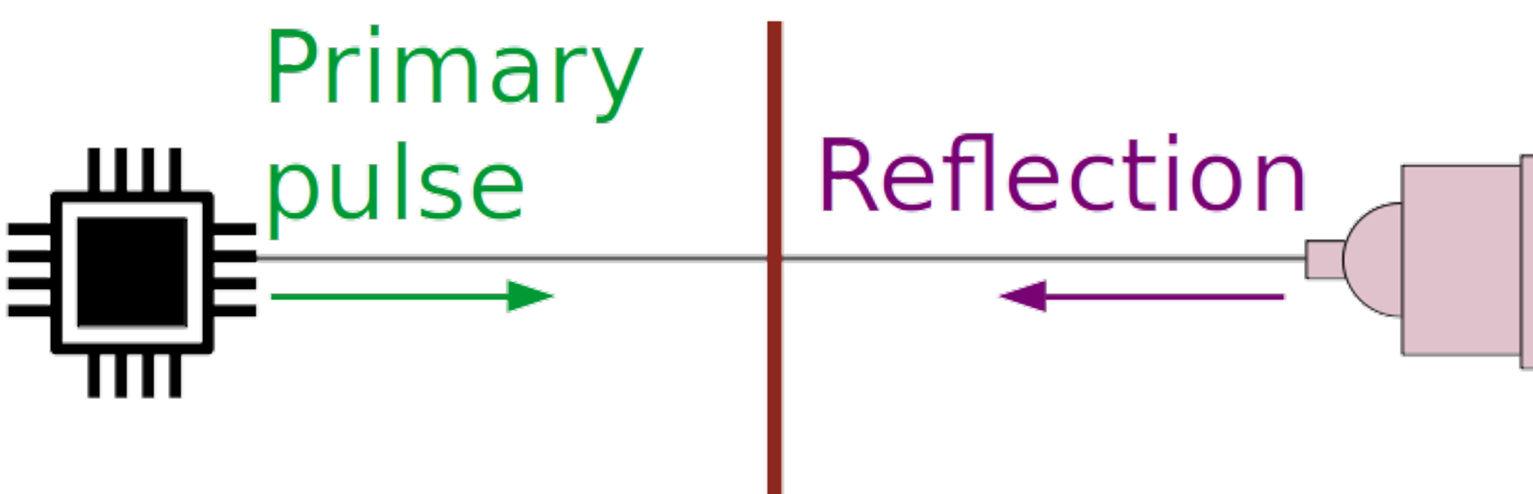
\includegraphics[width=1.1\textwidth]{commissioning/fig_commissioning/scheme_reflecto.pdf}
    \captionsetup{justification=centering}
    \caption{Normal reflection at PMT divider.
      \label{subfig:reflecto_normal}}

  \end{subfigure}
  \hfill
  \begin{subfigure}[b]{0.3\textwidth}
    \centering
    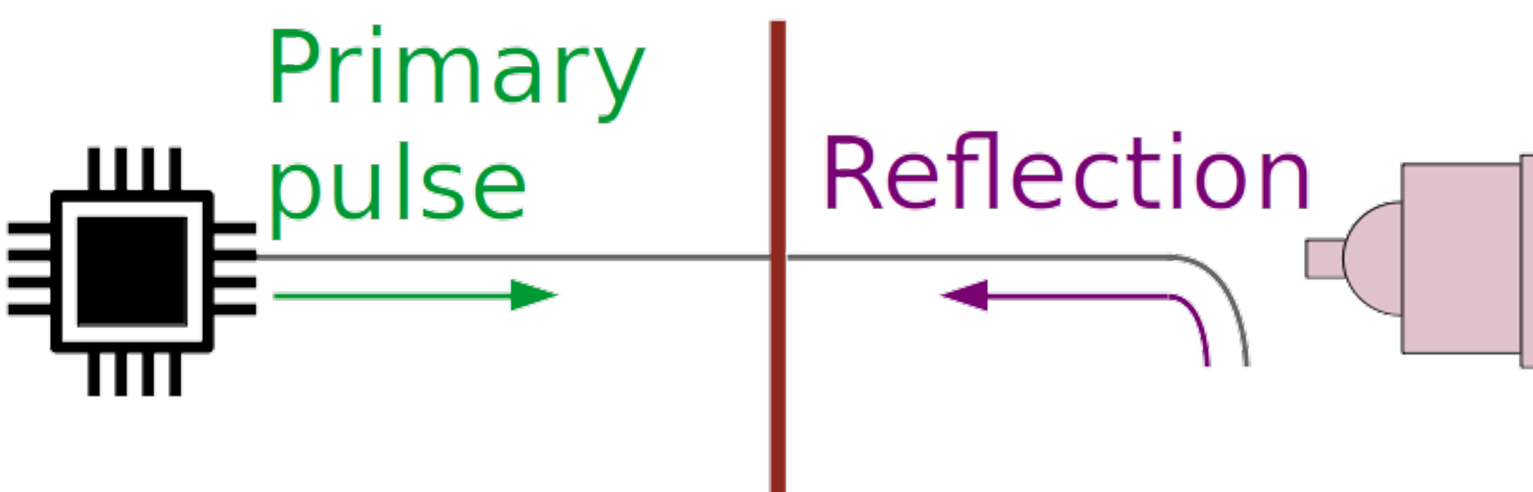
\includegraphics[width=1.1\textwidth]{commissioning/fig_commissioning/scheme_reflecto_1.pdf}
    \captionsetup{justification=centering}
    \caption{Cable not connected at PMT.
      \label{subfig:reflecto_pmt}}

  \end{subfigure}
  \hfill
  \begin{subfigure}[b]{0.3\textwidth}
    \centering
    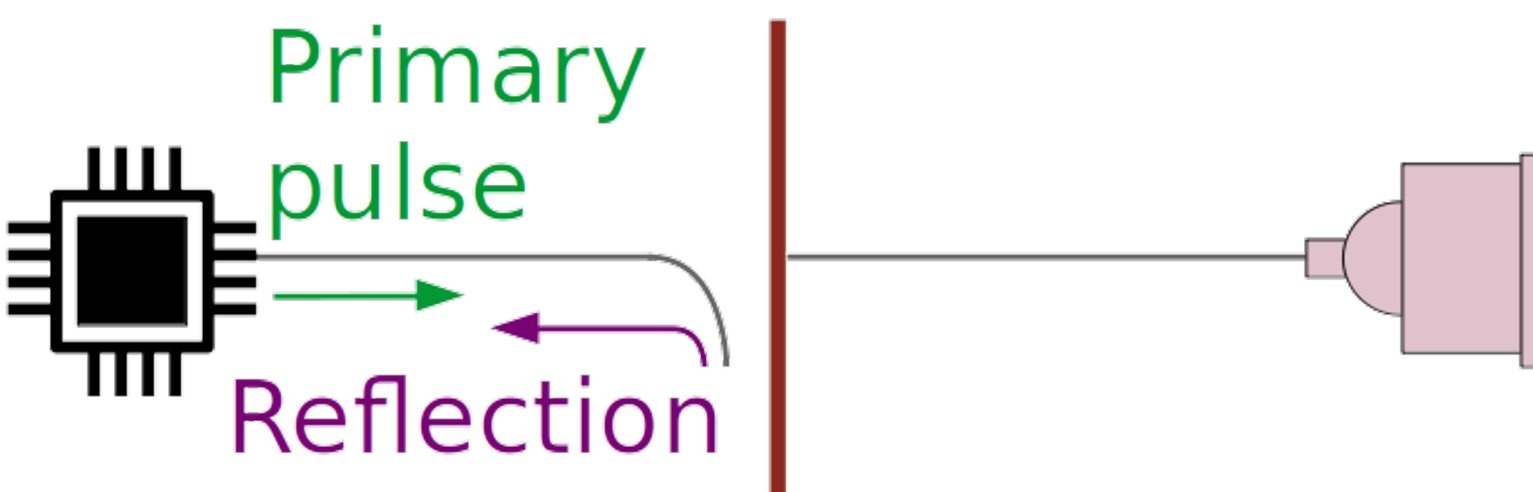
\includegraphics[width=1.1\textwidth]{commissioning/fig_commissioning/scheme_reflecto_2.pdf}
    \captionsetup{justification=centering}
    \caption{Cable not connected at patch panel.
      \label{subfig:reflecto_pp}}

  \end{subfigure}
  \caption{A representation of pulses sent in a cable for the reflectometry analysis is given.
    The electronic boards are symbolised by the black chip, and the patch panel by the red vertical bar.
    Three scenario where a primary pulse is sent in one cable (represented in grey), are represented.
    (a) The cable is well connected at the patch panel and at the PMT. The signal reflects at the PMT divider.
    (b) The cable is not connected at PMT and the signal is reflected at the end of the cable.
    (c) The cable is not connected at patch panel and the signal is reflected at the end of the external cable.\label{fig:reflecto_scheme}}

\end{figure}
Then the signal travels back from the PMT to the electronic board channel, where it is recorded by the acquisition.
We called this recorded reflected pulse \emph{secondary} pulse.
An example of the total recorded signal is displayed in Fig.~\ref{subfig:total_waveform}.
In order to accumulate enough statistics, we send thousands of pulses in each coaxial cable.
The analyses of the shape and of the arrival time of those secondary pulses for each channel is called \emph{reflectometry}, and allow us to check the coaxial cable conditions and to control their lengths.

\subsection{Pulse timing: controlling cable lengths}
\label{subsec:timing}

The first step of this analysis is to experimentally determine the length $l_{j}^{m}$ for all signal cables $j$ installed on the demonstrator.
This length is defined as
\begin{equation}
  l_{j}^{m}= 0.5\,t_{j}\,v_{p}\, ,
\end{equation}
where $t_{j}$ stands as the time made by the electrons to do a round trip between one electronic channel and one PMT, and $v_{p}$ is the velocity of electrons in the coaxial cables, which can be expressed as a fraction of light speed in vacuum, $c$.
The time difference $t_{j}$ between the primary pulse and the secondary pulse is written as
\begin{equation}
  t_{j} = \braket{t_{\text{secondary pulse}}-t_{\text{primary pulse}}}_{p} \, \text{,}
\end{equation}
$\braket{}_{p}$ being the average over all pulses sent in one single cable $j$.
The velocity $v_{p}$ is supplied by the cable manufacturer as
\begin{equation*}
  v_{p}=\frac{c}{\sqrt{\epsilon_{r}}}\,\text{,}
\end{equation*}
with $\epsilon_{r}$ the relative dielectric constant of the material.
Therefore, this celerity depends on the components.
For the coaxial cables chosen in the demonstrator design, the data sheet of the cable gives ${v_{p}=0.69\,c}$.
A study is performed to verify experimentally the value of $v_{p}$.
Three cables of different lengths are measured with a precision of $1$ cm.
A thousand of primary pulses are sent in each of the three cables, then the time for each secondary pulse is recorded.
At the end, we have three independent measures of the velocity $v_{p}$ in the used coaxial cables.
In Fig.~\ref{fig:celerity} is displayed the lengths $l_{j}$ as a function of the times $t_{j}$.
\begin{figure}[h]
  \centering
  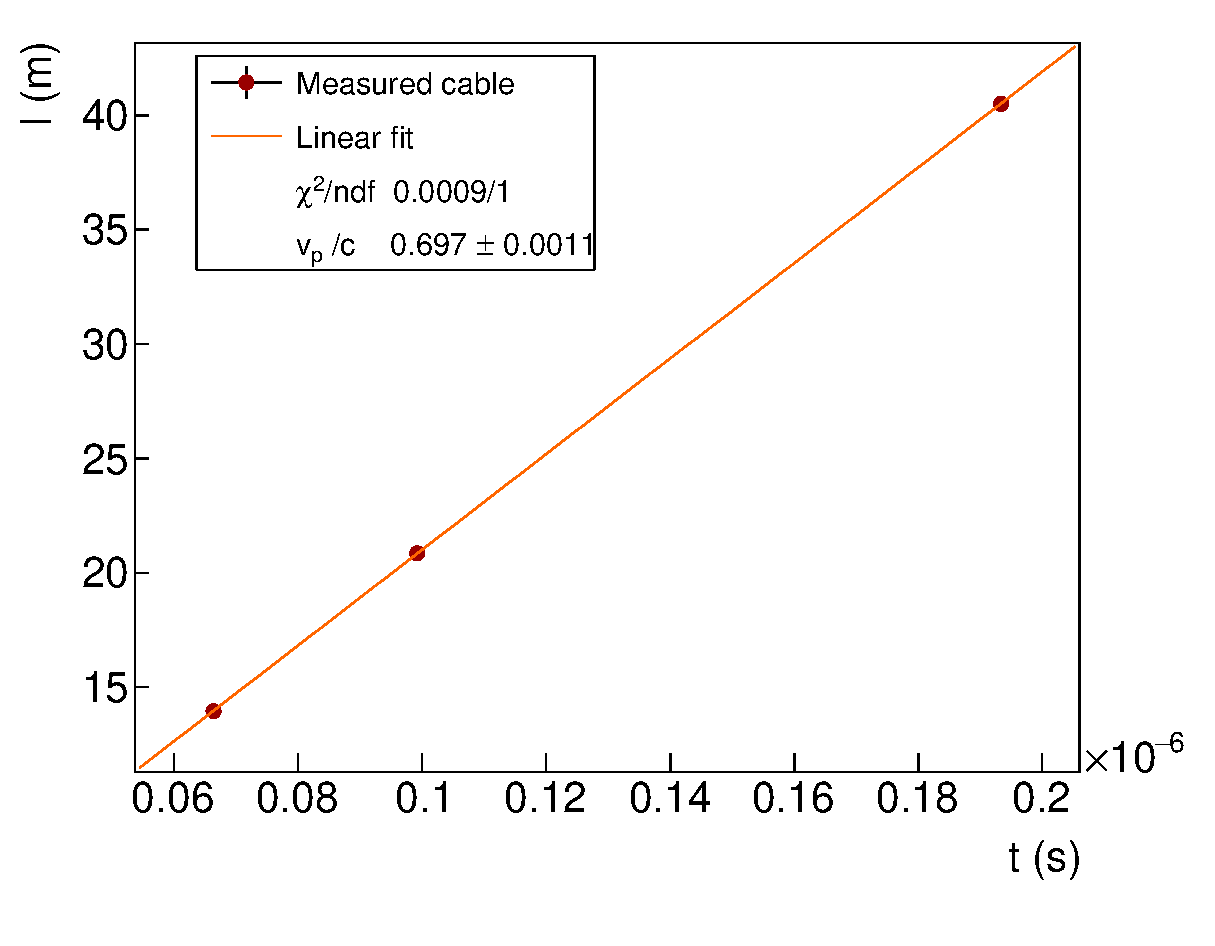
\includegraphics[width=15cm]{commissioning/fig_commissioning/celerity.eps}
  \caption{Three different lengths $l_{j}$ of cables are measured.
    Pulses are sent inside all cables.
    The lengths $l_{j}$ are plotted as a function of the time differences $t_{j}$ between primary and secondary pulses.
    The value of $v_{p}/c$ fitted from the data points is displayed.
    This value of $0.697\pm 0.0011$ shows the compatibility with the one supplied by the constructor, of $0.69$ c.
    \label{fig:celerity}}
\end{figure}
The fitted value of $v_{p}/c = 0.697\pm 0.0011$ is displayed and shows a compatibility up to $7\sigma$ with the data sheet.

As we want to determine the time interval $t_{j}$, we have to define what is the \emph{time} of a pulse.
In this analysis, we use a technique called Constant Fraction Discriminator (CFD), providing an amplitude-independent information about time of a pulse.
This algorithm aims at tracking a signal and defining its time arrival at a given fraction $f$ of its maximal amplitude.
The two main advantages of this technique is that it provides an efficient rejection of the noise in the acquisition window, and gives a good resolution on the measured time.
Nevertheless, the possible influence of the chosen value for the $f$ parameter on this time resolution has to be investigated.
We perform such a study in Sec.~\ref{subsec:CFD}.
We concluded that the highest precision on the time measurement arises for $f = 40\%$, and we adopt this value for the following analysis.
A graphic representation of the CFD time search is given in fig.~\ref{subfig:zoom_secondary}.
\begin{figure}[h]
  \centering
  \begin{subfigure}[t]{0.7\textwidth}
    \centering
    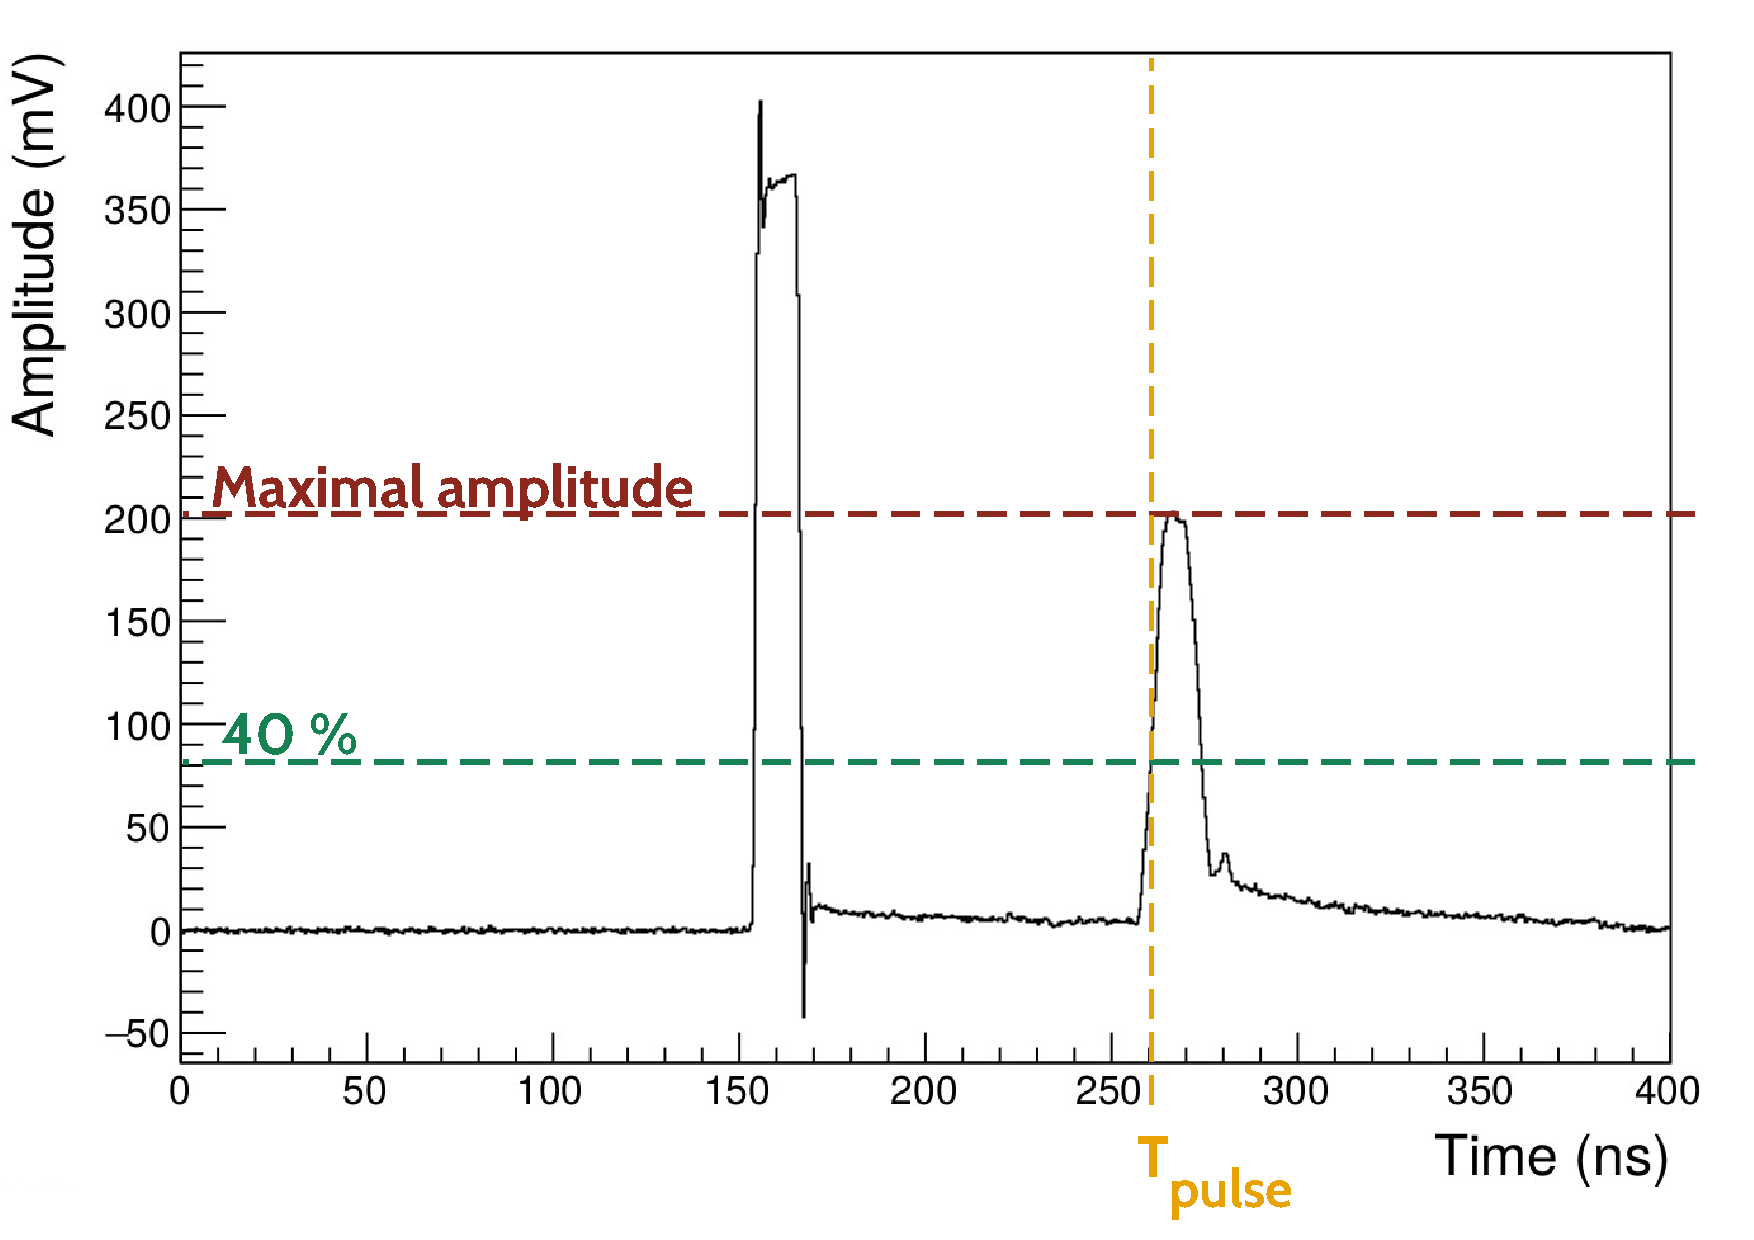
\includegraphics[trim={1.2cm 3.5cm 1.7cm 3.1cm},clip,width=1\textwidth]{commissioning/fig_commissioning/CFD_example.pdf}
    \captionsetup{justification=centering}
    \caption{Total recorded waveform
      \label{subfig:total_waveform}}
  \end{subfigure}
  \hfill
  \begin{subfigure}[t]{0.7\textwidth}
    \centering
    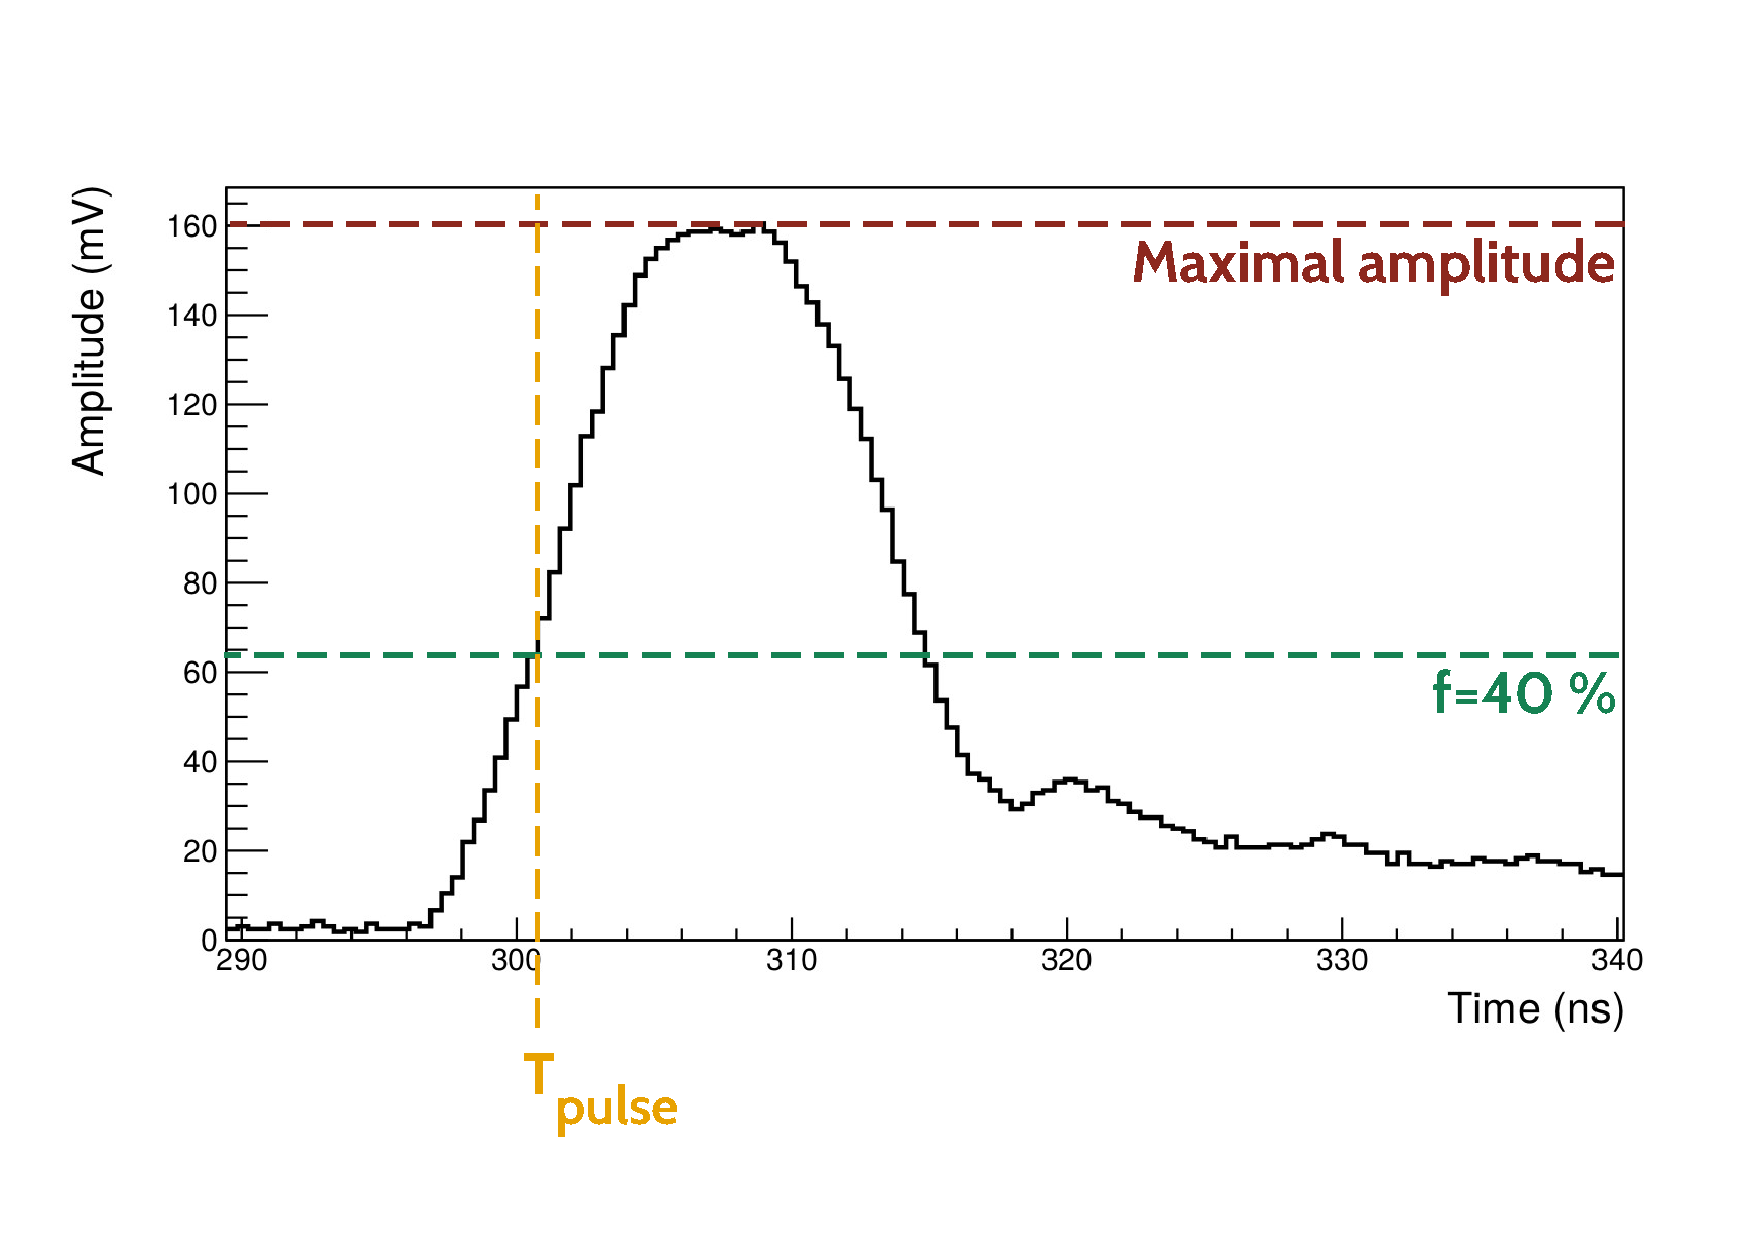
\includegraphics[trim={1.2cm 1.5cm 1.7cm 3.1cm},clip,width=1\textwidth]{commissioning/fig_commissioning/CFD_example_zoom.pdf}
    \captionsetup{justification=centering}
    \caption{Zoom on secondary pulse
      \label{subfig:zoom_secondary}}
  \end{subfigure}
  \caption{(a) Total recorded waveform: primary pulse (left) and secondary the pulse (right).
    (b) Zoom on the secondary pulse.
    A representation of time computed with a Constant Fraction Discriminator (CFD) is provided.
    Its maximal amplitude (red dotted line) and its fraction for $\text{f}=40\%$ (green dotted line) are displayed.
    The time $\text{T}_{\text{pulse}}$ (orange dotted line) represents the time of arrival of the secondary pulse computed with CFD, with the fraction $\text{f}=40\%$.
    \label{fig:CFD}}
\end{figure}
As we want to measure the installed cable lengths $l^{m}_{j}$, and compare them to the initially designed ones, $l^{d}_{j}$, we define the length difference $\Delta L_{j}$ as:
\begin{equation}
  \Delta L_{j} = l^{m}_{j}-l^{d}_{j}\, .
\end{equation}
In Fig.~\ref{fig:LengthDiff} is displayed the distribution $\Delta L$ for all the measured lengths.
\begin{figure}[h]
  \centering
  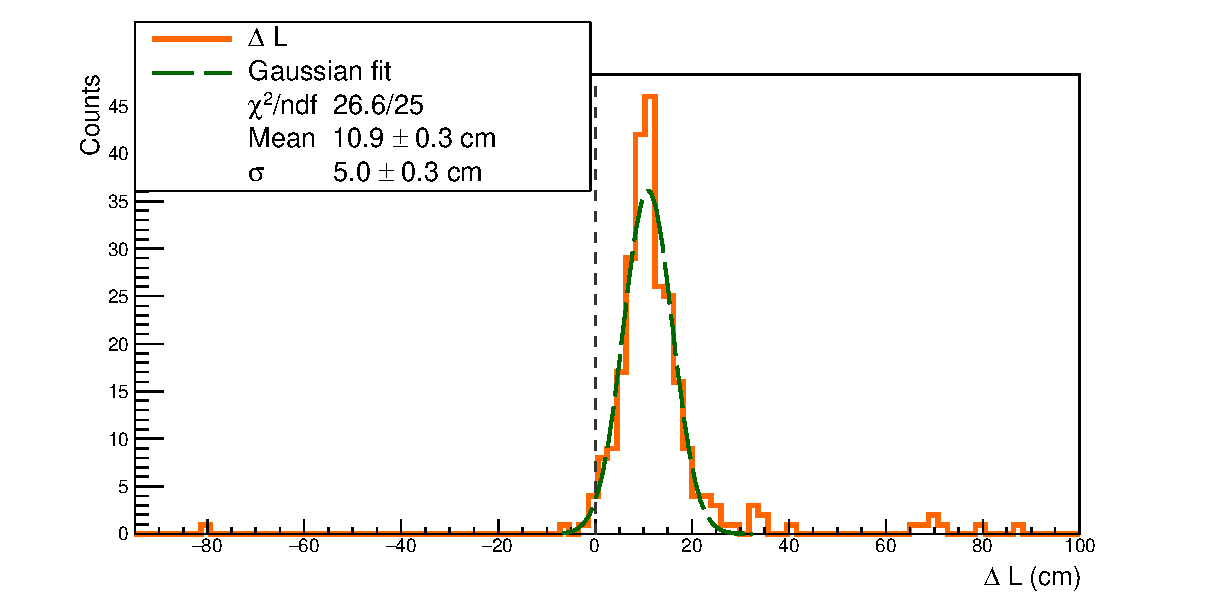
\includegraphics[width=15cm]{commissioning/fig_commissioning/length_diff.eps}

  \caption{The distribution of difference between the measured lengths $l^{m}$ and the expected lengths $l^{d}$ is displayed in orange solid line.
    The black dashed line represents the case where $l^{m}_{j} = l^{d}_{j} \;\forall j$.
    The Gaussian fit (green dashed line) presents a mean of $10.9 \pm 0.3$ cm.
    Some data points considered as outliers are beyond $3\sigma$.
    \label{fig:LengthDiff}}
\end{figure}
In hypothetical perfect conditions, all the cables should fit the design length, in other words, $l^{d}_{j} = l^{m}_{j}$.
Consequently the $\Delta L$ distribution should a peak at zero, as materialised by the black dashed line.
However, in real conditions, the measured length can be different from the designed one, leading the $\Delta L$ distribution plotted in orange solid line.
We conclude that the observed cable length $l^{m}$ differs from $l^{d}$ by $+10.9\pm 0.3$ cm, meaning that cables are longer than expected in average.
This may reveal a bias coming from the device used to cut the cables.
In fact, during cable cutting work, we noticed that the cutting device had a tendency to slip, probably leading to cables with extra lengths.
We assumed the cutting device has a given probability to slip for one meter of cable.
If this is the case, the probability for the device to give extra length should increase with the cable length.

To verify this assumption, we plot in Fig.~\ref{fig:CutBias} the length difference $\Delta L$ as a function of the initial design length $l^{d}$ (cyan).
From those data points, we compute a linear fit (orange solid line), parameterised as $y = \alpha x + \beta$, revealing that the cutting device presents two different biases.
\begin{figure}[h]
  \centering
  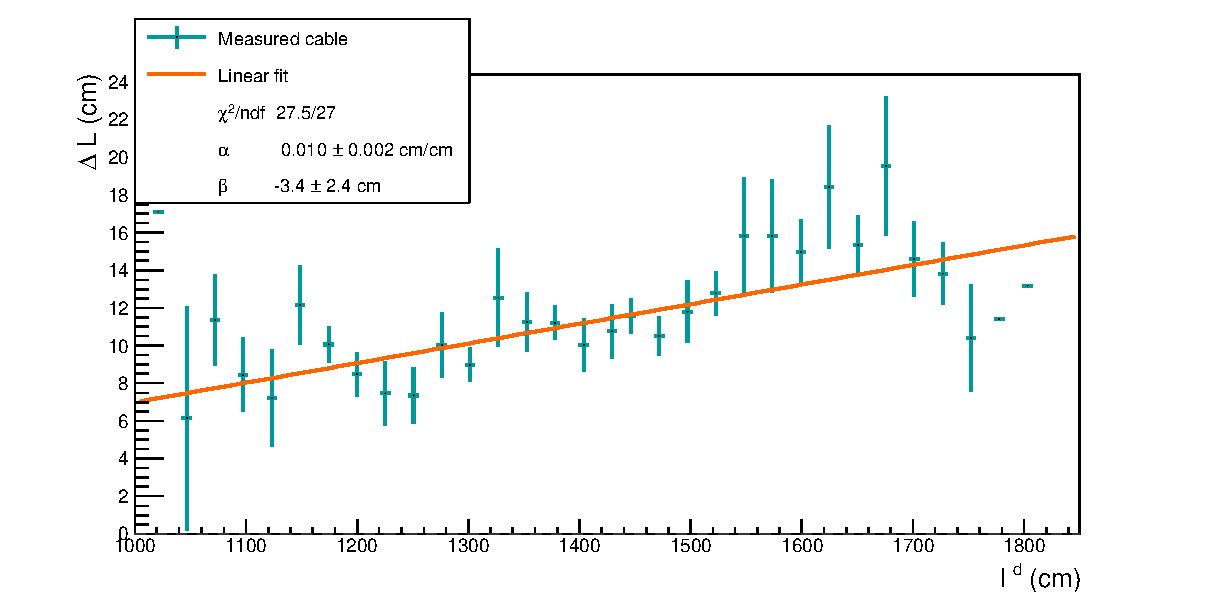
\includegraphics[width=15cm]{commissioning/fig_commissioning/cut_biais.eps}

  \caption{$\Delta L$ is plotted with $l^{d}$ (cyan), where $l^{d}$ is averaged for all the lengths designed to have the same value, being at the origin of vertical error bars.
    In black dashed line is represented the case where $l^{m} = l^{m}$.
    Data points are fitted by $\alpha x + \beta$, with $\alpha > 0$ and $\beta < 0$, revealing the two biases of the cutting device.
    \label{fig:CutBias}}
\end{figure}
The value of $\beta$ shows that the cutting device systematically took away $3.4$ cm of each cable.
Nevertheless, as the shortest cable was designed to be 10 meters long, there are no important consequences of this bias on the length difference $\Delta L$.
Besides, the slope $\alpha = 0.010\pm 0.002$ of the linear fit reveals that the cutting device adds one centimetre for every meter of cable, being compatible with the hypothesis on the cutting device sliding.
Hopefully this bias is not problematic as it makes most of the actual cable lengths longer than the design, while shorter lengths could have lead to systematic connection issues to PMTs.
However, we notice that a few cables have been cut too short by mistake, the worse of them being $80$ centimetres shorter than expected.
Fortunately, this cable  was successfully connected to PMT despite this deficit.
On the contrary, few cables have a large extra length.
This probably is due to human punctual mistakes on top of the observed bias, but without any strong consequences for the calorimeter operation.
In conclusion, no important mistakes have been made when cutting cables, and we had no issue for connecting the only problematic cable.

If the main goal of this study is to check the lengths of coaxial cables, it also aims at correcting the time of recorded events, from the time made by the signal to travel from a PMT to an electronic channel.
taking into account the time for the signal to travel through cables.
This become possible with the reflectometry study we performed.
Knowing real lengths of cables and using the celerity of the signal, we deduce the time needed for the signal to travel from one given PMT divider to the electronic boards.
Then we can correct event times.

As explained previously, the time $t_{j}$ gives information about the length of the cable $j$.
We remind the coaxial cables are divided in two parts, one external and one internal, both linked by the so-called patch panel.
Thus we can use that travel time to detect possible disconnection of a cable at patch panel.
In fact, if one cable is not connected at the patch panel -- this case is illustrated in Fig.~\ref{subfig:reflecto_pp}, -- the pulse reflects at the end of the external cable part, going back to the electronic board.
This very short time, giving information about the location of the reflection, is used to tag a patch-panel disconnection.
Then, a simple check onsite can confirm this observation, and the external part of the cable can be connected to the patch panel.\\

This study allowed us to control and record the lengths of all coaxial cables installed on the SuperNEMO demonstrator at LSM, and gave information on the status of cable connections at patch panel.
We also have understood the main results on measured cable lengths and the functioning and biases of the cutting device that we used.

\subsection{Signal attenuation}
\label{subsec:attenuation}
The attenuation of an electric signal is a problem common to all electronic fields, and comes from the charge loss of an electromagnetic wave travelling in a medium.
%% Then, another test for controlling the cable condition is to check if this attenuation matches
%% the expectations (i.e. the attenuation per metre of cable given by constructor).
%% The signal attenuation car be define in two different ways:
%% \begin{itemize*}
%% \item using the signal amplitude ratio
%% \end{itemize*}
For a coaxial cable, this attenuation mainly depends on the signal frequency $f$ in MHz and on the cable characteristics.
For the coaxial cables, the theoretical linear attenuation $\alpha_{\text{att}}^{\text{th}}$, so be it the attenuation by metre of cable in dB/m, is supplied by the constructor as
\begin{equation}
  \alpha_{\text{att}}^{\text{th}} = f\sqrt{\epsilon}(\frac{a}{\sqrt{f}}+b)\,,
\end{equation}
where the factor $a$ depends on the diameter of the dielectric material on one side, and of the diameter of the conductor material on the other side, and where $b$ is function of the dielectric loss factor, characterising the material's dissipation of electromagnetic energy.
For the used coaxial cables, and with a frequency $f$ of few GHz for the signal pulses sent in cables, we calculate this attenuation as $\alpha_{\text{att}}^{\text{th}} = 1.22$ dB/m.
In a more general manner, the attenuation of a signal in dB is defined with the decimal logarithm of a power ratio.
We use this definition to determine the attenuation in the framework of the reflectometry analysis, defining the attenuation $\mathcal{A}$, for a given length of cable $l$, as
\begin{equation}
  \mathcal{A}=10\log_{10}\frac{V_{\text{primary pulse}}}{V_{\text{secondary pulse}}} \,\text{,}
\end{equation}
where $V_{i}$ is a quantity representing the intensity of the signal.
$V$ can correspond to the maximal amplitude of the pulse, as well as the \emph{integrated charge} of the pulse, defined as the amount of current received by the acquisition over a given time window.
As the provided data sheet does not specify the attenuation of which quantity (amplitude or charge) represents $\alpha_{\text{att}}^{\text{th}}$, we decide to investigate both in the following.
Then, we define the linear attenuation $\alpha_{\text{att}}^{\text{R}}$, measured by reflectometry in dB/m, with
\begin{equation}
  \mathcal{A} = f_{r}+\alpha_{\text{att}}^{\text{R}}\,l\,,
\end{equation}
with $f_{r} = -10\log_{10}R$, where $R$ is the reflection factor characterising the pulse reflection on the PMT divider.
In fact, as the circuit is opened, the pulse is reflected at the PMT divider, but only partially.
A part of the signal is not reflected but lost through the divider.
This reflection is characterised by $R$, which is function of the impedance $Z_{c}$ of the cable, and of the impedance $Z_{d}$ at the divider level, where the pulse is reflected.
It is written as
\begin{equation}
  R = \frac{Z_{d}-Z_{c}}{Z_{d}+Z_{c}}\,,
\end{equation}
where we have the limit
\begin{equation}
  \lim_{Z_{d} \to \infty} f_{r} = 0 \text{ and } R=1\,,
\end{equation}
expressing a total reflection occurring when the impedance at the PMT divider is infinite.
The main goal here is to determine the value of $\alpha_{\text{att}}^{\text{R}}$, using the reflectometry data, and to compare it with $\alpha_{\text{att}}^{\text{th}}$.
Moreover, the impedance $Z_{d}$ value at PMT divider can be estimated from the determination of $f_{r}$.
In Fig.~\ref{fig:attenuation} is shown the linear dependence between the attenuation $\mathcal{A}$ and the cable length $l$, and two data set are presented.
The cyan scattered markers represent the attenuation calculated from the amplitude ratio $A_{\text{primary pulse}}/A_{\text{secondary pulse}}$, and the magenta markers correspond to the attenuation calculated from the charge ratio $Q_{\text{primary pulse}}/Q_{\text{secondary pulse}}$.
The amplitude $A_{i}$ is given in mV and the charge $Q_{i}$ in mV.ns.
\begin{figure}[h]
  \centering
  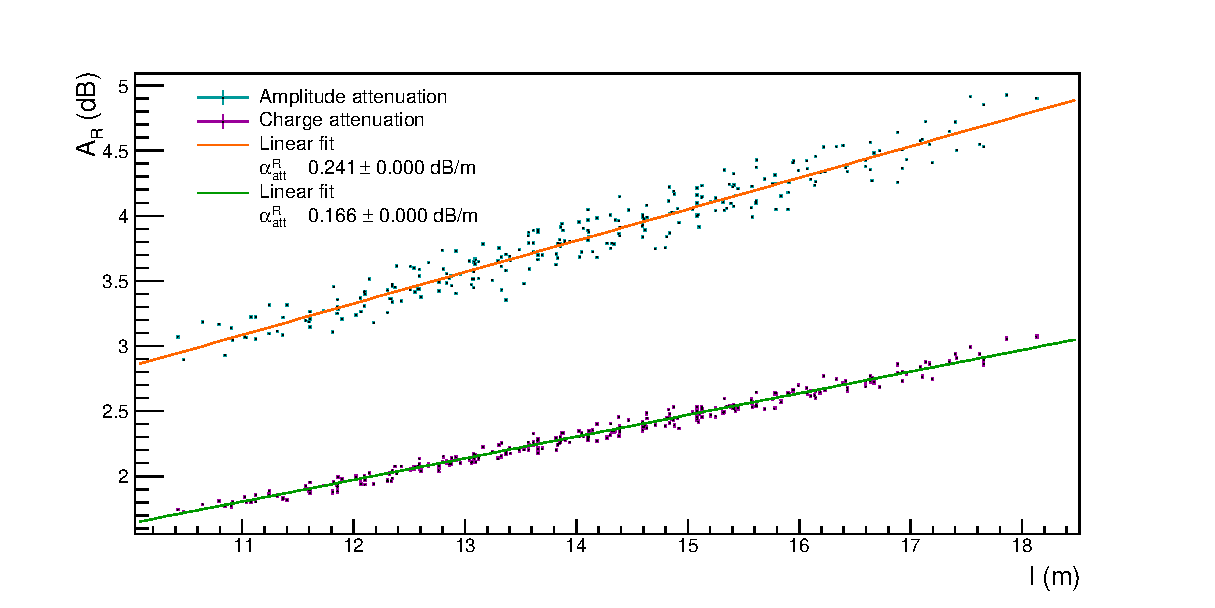
\includegraphics[width=15cm]{commissioning/fig_commissioning/attenuation_length.eps}
  \caption{The amplitude $\mathcal{A}$ is displayed as a function of the measured cable length $l$.
    The data set calculated with the amplitude (charge) is given in cyan (magenta) and fitted by a linear function in orange (green).
    The values of the slope, which represent the linear attenuation of the coaxial cables in dB/m, are respectively $\alpha_{\text{att}}^{\text{R, amp}} = 0.241\pm 0.000$dB/m and $\alpha_{\text{att}}^{\text{R, ch}} = 0.166\pm0.000$dB/m.
    The two $y$-intercept values, which represent the reflection of the pulse on the PMT divider, are $f_{r}^{amp} = 0.402\pm 0.032$ dB and $f_{r}^{ch} = -0.020\pm 0.013$ dB.
    \label{fig:attenuation}}
\end{figure}
The values of $\alpha_{\text{att}}^{\text{R}}$ and $f_{r}$, for both amplitude and charge cases, are displayed in the legend.
Firstly, the two linear fits reveal that, whether calculated with the amplitude, or with the charge, the linear attenuation $\alpha_{\text{att}}^{\text{R}}$ is smaller than the calculated one $\alpha_{\text{att}}^{\text{th}}$ (for the amplitude case, $\alpha_{\text{att}}^{\text{th}}\simeq 5\times \alpha_{\text{att}}^{\text{R, amp}}$, and for the charge case $\alpha_{\text{att}}^{\text{th}}\simeq 7\times \alpha_{\text{att}}^{\text{R, ch}}$).
That means the signal is less affected, when transmitted by the cable, than expected.
Secondly, the attenuation in charge is less important that the attenuation in amplitude.
This can be easily explained: as it is integrated over time, the charge is a quantity less affected by amplitude variations that the amplitude itself.
For the same reason, the charge data set points are less spread than the amplitude ones, meaning that we are less sensitive to cable length variations when using the charge quantity.


This work achieved, we want to verify if no cable was damaged after installation.
Reflectometry also aimed at checking cable conditions by performing waveform shape analysis on secondary pulses.

\subsection{Pulse shape analysis}
\label{subsec:pulse_shape}
In Fig.~\ref{fig:CFD} is displayed an example of \emph{normal} pulse, which corresponds to the case represented in Fig.~\ref{subfig:reflecto_normal}.
In this case, the pulse sent in the cable travels to the PMT, and goes back to the acquisition after reflection on the divider.


\subsection{Comparison with $^{60}$Co}

\subsection{Conclusion}
A faire : regarder le rising time en fonction de la longueur du cable\\
Regarder la différence de temps de montée du signal sur deux PMs très éloignés

\section{Calibrating the electronic boards}
\label{sec:TimeSynchroFEB}

\subsection{Principle}
\subsection{Measuring the time offset of front end boards}
\subsection{Results}


\section{Energy calibration of optical modules}
\label{sec:comm_energy_calibration}


*thèse Arnaud page 103*

As described in Sec.~\ref{subsec:OMtimeResponse}, the collected charge at PM voltage divider is proportional to the amount of incident photoelectrons, and then to the initially deposited energy inside the scintillator.
Once optical modules were assembled (optical coupling, packing, shielding integration), they were individually tested at Bordeaux laboratory, CENBG, with an electron spectrometer [ref].
Their energy resolutions for $1$ MeV-electrons at the centre of scintillator front face were determined.
High voltages were set to optimal values, to obtain an amplitude of $300$ mV for $1$ MeV electrons.
However, after calorimeter integration, due to different environment, amplitude spectra of each optical block have to be re-aligned.
This work was performed by Axel Pin, PhD student at CENBG.
We give in this section a summary of this energy calibration study.

*A finir\\




\section{Baseline studies}
\label{sec:comm_baseline}

\section{Light Injection System}
\label{sec:LI}
